\documentclass{article}
\usepackage[utf8]{inputenc}

\usepackage[english]{babel}
\usepackage{amsthm}
\usepackage{amssymb}
\usepackage{mathcomp}
\usepackage{amsmath}
\usepackage{natbib}
\usepackage{array}
\usepackage{wrapfig}
\usepackage{multirow}
\usepackage{tabularx}
\usepackage{multirow}
\usepackage{graphicx}
\usepackage{geometry}
\usepackage{multicol}
\usepackage{blindtext}
\setlength{\columnsep}{1cm}
\usepackage[rightcaption]{sidecap}
\linespread{1.6}

\newcommand{\pic}[2]{\begin{figure}
  \centering
  \includegraphics[width=0.9\textwidth]{#1}
  \caption{#2 }
  \label{fig:#1}
\end{figure}}

\title{Final Report}
\author{Jingyuan Chen, Sean Eva}
\date{May 2022}

\begin{document}

\maketitle

\pagebreak
%Abstract

During this project we learned all about Neural Networks. We started from the beginning and learned about the way that neural networks are designed based on the way the brain works and processes information. Then we used this information that we learned to implement basic neural networks on different data sets of various complexities. In order to test our abilities using neural networks we wanted to use increasingly more complex data sets so that we can check for different areas for improvements. The data sets we worked with are the MNIST Database of handwritten Digits, Chars74k data set on characters, and the Petals to the metal data set on flower classification. We will then compare the effectiveness of our neural networks against the abilities of other analysis methods that we learned in the class such as Linear Discriminant Analysis (LDA), Quadratic Discriminant Analysis (QDA), and K-Nearest Neighbors (KNN) just to name a few examples. This will test our abilities to not only learn and implement neural networks but also our abilities to accurately compare it against other methods that we have learned during this semester.

\pagebreak
%Main Content

\begin{multicols}{2}

Briefly, we learned about neural networks for the first time during this project. We learned about the basic structure and different types of neural networks: artificial, recurrent, and convolutional. Artificial neural networks work in a straight line where an input is taken in and processed through each layer individually until it reaches an estimated output after going through each layer once. A recurrent neural network is similar to artificial neural networks, but it is able to reuse layers more than once to analyze the data. And lastly, a convolutional neural network breaks up the data into different convolutional layers that will all be analyzed separate;y and then put back together to formulate an output. Convolutional neural networks are most commonly used in image data analysis and so that is what we will use most often in this project. Additionally we primarily used the the Python package Tensorflow developed by Google instead of Pytorch from Facebook to run our neural networks.\\
We also applied what we have learned about neural networks to three different data sets, each of increasing complexity. We started by working with the simple, iconic data set for learning about neural networks, the MNIST data set. For example, Tensorflow included a learning article to introduce beginners to tensorflow and neural networks that use the MNIST data set. Then we used the Chars74k data set. And finally we used a Kaggle data set on flower images called Petals to the Metal. Each of these data sets are over images of their respective items. Additionally, since these data sets are all about images, we will be focusing on using convolutional neural networks since those are the best option to use when it comes to image processing. Sean focused primarily on a lot of the more simpler neural networks to MNIST and applying methods like LDA, QDA, and KNN to the data sets to compare the performance against the methods that we learned in the class. Then Jingyuan focused on creating and implementing the much more complex neural networks and the dimension reduction for the more complex Chars74k and Petals to the Metal data sets.

\section*{Data Structure}

Starting with the MNIST data set. Each image is $28 \times 28$ pixels. This was a good size for us to practice with and an ideal size for our other data sets that we are working with to be formatted into as it will make it much more simple. For the Chars74k data set, we opted to use the EnglishImg file which provided segmented characters from the English alphabet and numbers from natural scenes, such as those that you would find on a building, on a sign, or anywhere else in real life. Each of these images were different sizes so we first wanted to format each of these so that each image was the same size as each other. Lastly, for the Petals to the Metal data set, the images were all $192\times 192$ for 12753 training samples and xxx val files. With this size it is of orders of magnitude larger than our MNIST or Chars74k data sets. This means that we will need to reduce these their sizes. Additionally, this data set does not provide test labels for the test images so we need use val files instead of the testing set to obtain a testing accuracy.

\section*{Data Pre-Processing}

For the MNIST data set, the default size of the image to process of $28\times 28$ which will create a feature vector of size $28*28 = 784.$However, as our data set become more complex, due to our hardware limitation on our devices, namely the available memory of the computer, we need to crop the images from the data sets. We tried different options for formatting the larger images from Chars74k as $32\times 32, 64\times 64, 96\times 96$, as well as other sizes. In addition to formatting the size, we also tried to remove coloring of the images. We ended up using the reduced size of $64\times 64$ and kept the colors from the images. The inclusion of colors expands the complexity of this data set by $3$ which means that this data has the shape $64 \times 64\times 3$ and we normalized it using \textsc{cv2} from opencv. We then applied this same method for the Petals to the metal data set as well to create a standard for those more complex data sets. When we want to use these methods in class, we stretch the data set. We flatten the data set into a feature vector of length $28\times 28 = 784$ for the MNIST data set. For the complex color images from Chars74k and Petals to the Metal, we also used the \textsc{cv2.cvtColor} to convert it to gray-scale and then resize it to $28\times 28$ as we did in class. Examples of this pre-processing can be seen in figure \ref{fig:FlowerDataSet}.

\section*{Building the Data Set}
To convert the images and labels into a more proper data set with labels attached to images by using \textsc{tf.data.dataset}. We then shuffled the data set and chose a batch size of 64.


% \begin{figure}
%   \centering
%   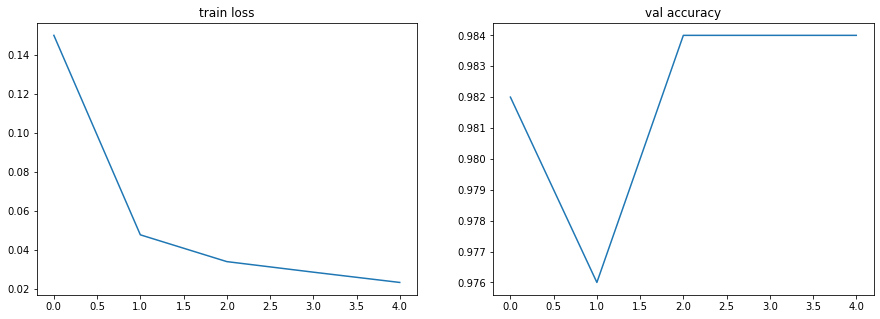
\includegraphics[width=0.9\textwidth]{NumPlot3.png}
%   \caption{The train loss and val accuracy}
%   \label{fig:NumPlot3}
% \end{figure}

\section*{Analyzing the Data}
We use convolution neural network (CNN) for the MNIST data set. The neural network contains two convolution layers and two fully connected layers. We choose RELU as the activation function, Adam as the optimizer, and categorical-crossentropy as the loss function. Categorical-crossentropy computes cross entropy loss between the labels and predictions. By training five times, performing five epochs, we found the test accuracy reached about $98.9\%$. We also applied LDA, QDA, KNN, RandomForest, and SVM to compare the accuracy between the neural network and the methods learned in class. As can be seen in figure \ref{fig:NumPlot1}, the accuracy between the CNN is very close to the accuracy of KNN, random forest, and SVM, the CNN performs slightly better than LDA and significantly better than QDA. Then in figure \ref{fig:NumPlot2} we demonstrate the ability of the CNN to predict what a number character is, and since it has a high degree of accuracy, we see that it does not make any mistakes in making predictions for what the number digits are.\\\\\\\\
For Chars74 data set, we used the same CNN model, we designed a early stop when our val loss has changed below 0.02 for 10 times. After 24 epoch, we achieved $60\%$ testing accuracy. We also applied LDA, QDA, KNN, RandomForest and SVM just like we did on MNIST. With the more complex data set, we found the LDA did not perform nearly as well and this can be seen in figure \ref{fig:CharsPlot1}.\\

Moreover, with increasingly more complex data sets, we would like to use more complex neural network to see if it can improve the performance. We applied the network which modify by AlexNet and it reach $65\%$ accuracy by 17 epochs. And we also tried the pre-trained DesNet121 model, which was able to achieve $80\%$ accuracy.\\
\end{multicols}

\begin{figure}
  \centering
  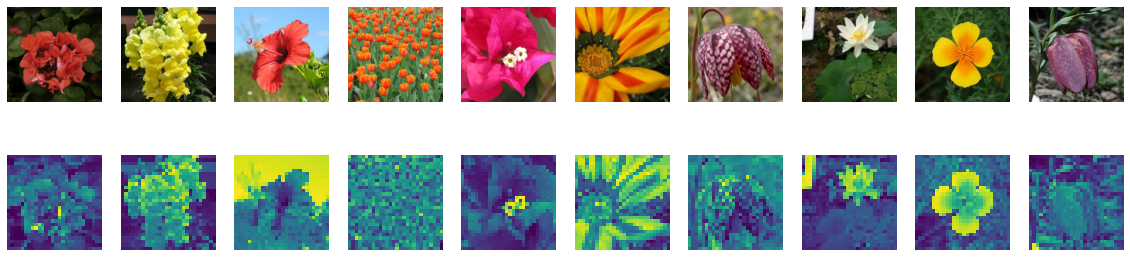
\includegraphics[width=1\textwidth]{FlowerData.png}
  \caption{This figure shows a sample of what happened to the flower images that we are using when we processed them into gray-scale and resized them. As can be seen, they are very small, pixelated images and they are also hard to see in gray-scale.}
  \label{fig:FlowerDataSet}
\end{figure} 
\begin{figure}
  \centering
  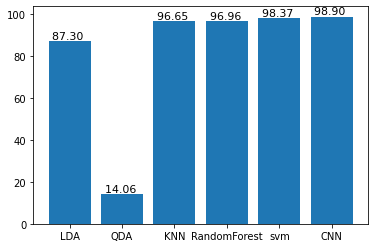
\includegraphics[width=0.6\textwidth]{NumPlot1.png}
  \caption{Bar graph comparing the accuracy of LDA, QDA, KNN, Random Forest, SVM, and CNN plotted against each other. We can see that KNN, Random Forect, SVM, and CNN are all very similar in performance with a slightly worse performance from LDA and significantly worse performance from QDA.}
  \label{fig:NumPlot1}
\end{figure}
\begin{figure}
  \centering
  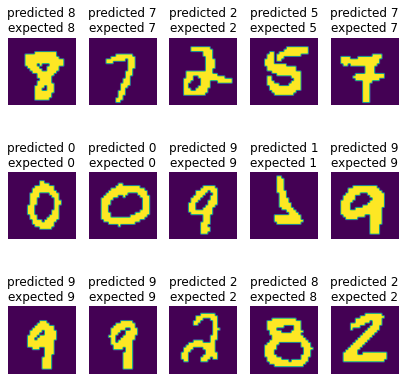
\includegraphics[width=0.50\textwidth]{NumPlot2.png}
  \caption{This is a diagram that shows the expected and predicted outcomes from the neural networks. From this we can see that the neural network had a high degree of accuracy as applied to this set of samples.}
  \label{fig:NumPlot2}
\end{figure}

\begin{multicols}{2}

\end{multicols}

\begin{figure}
  \centering
  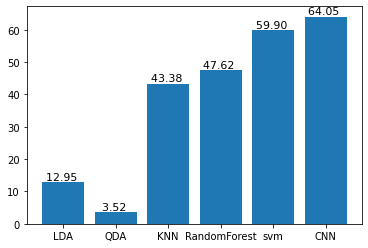
\includegraphics[width=0.65\textwidth]{CharsPlot1.png}
  \caption{Bar graph comparing the accuracy of LDA, QDA, KNN, Random Forest, SVM, and CNN plotted against each other. We can see that KNN, Random Forect, SVM, and CNN are all very similar in performance with a slightly worse performance from LDA and significantly worse performance from QDA.}
  \label{fig:CharsPlot1}
\end{figure}

\begin{multicols}{2}

\end{multicols}

\begin{multicols}{2}
For Petals to the Metal data set, we used the same CNN model as we used on the MNIST data set, After 6 epochs, we got $25\%$ testing accuracy. We again applied LDA, QDA, KNN, RandomForest, and SVM. Figure \ref{fig:FlowerPlot1} shows that our neural network is more accurate than these other methods. While none of the methods are nearly as accurate as they were when working with MNIST or even Chars74k, we still see that the CNN is our most beneficial option when it comes to analyzing this data. However, $25\%$ testing accuracy is very low for modern neural network. The reason that the test accuracy is very low is because our CNN model with the MNIST data set is too simple for this very complex data set. Hence we built more complex neural networks to see the performance. However, since the data set is very complex, if we make the neural network complex, such as adding a large number of convolutional layers, this will lead to a significant increase in training time, and we obviously do not want to spend a day or more to train our model. So we need a solution to shorten the training time. We tried converting the images directly to gray-scale to reduce the complexity of the data set, so we could use a simpler neural network to make predictions, but that didn't lead to particularly desirable improvements. Particularly when trying to simplify the data more than we already were (when reducing it), we ran into increased amounts of mistakes are made and our testing accuracy would decline. While there is some good trade-off in decreasing run-time, we do not want to sacrifice anymore accuracy from the little that we already have. So we started to use clients that allowed us to utilize our computers' graphics processing units (GPU) instead of just he computers' CPUs. Since we are making predictions on images, in this case, the GPU itself is dedicated to image processing, so using the GPU will be more suitable for model training and achieve acceleration. Due to equipment reasons, we used GPU mode on Google Colab for training, and we have adopted VGG13, VGG15, VGG19, and other models. For training, we build VGG13, the VGG15 model is based on the VGG19 model with some convolutional layers removed. By using the GPU, we got the test accuracy of these models, where we found that complex models will increase our accuracy, but if the model is too complex, it may lead to overfitting which is not good.
\end{multicols}

\begin{figure}
  \centering
  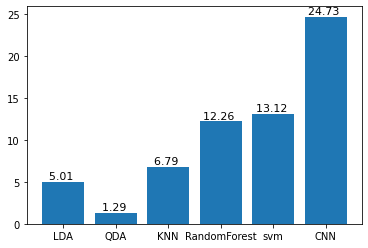
\includegraphics[width=0.65\textwidth]{FlowerPlot1.png}
  \caption{This is a bar graph that shows a side by side comparison of the performance of the CNN on the Petals to the Metal data set.}
  \label{fig:FlowerPlot1}1
\end{figure}

\begin{multicols}{2}

\end{multicols}

\begin{figure}
  \centering
  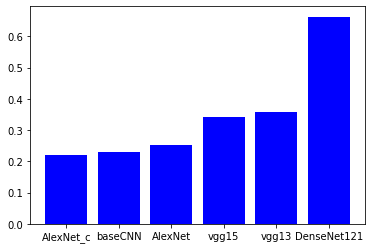
\includegraphics[width=0.65\textwidth]{FlowerPlot2.png}
  \caption{This is a bar graph showing the effectiveness of using the different types of neural networks that we used once we started using our GPUs to perform more complex neural netowrks.}
  \label{fig:FlowerPlot2}
\end{figure} 

\begin{multicols}{2}
Overall, by comparison we find that when our data set becomes more complex, the performance of the neural network is significantly higher than that of the methods we learned in the classroom. For example, in the relatively simple MNIST data set, the method we learned in the class Support Vector Machine (SVM) can also achieve a high rate of 98.4\%, the same as the neural network. But when the data set becomes more complex, such as the Chars74k data set, the SVM can only reach 56.8\$ accuracy, but the most basic CNN can also achieve $60\%$, and some advanced neural networks, such as the modify by AlexNet, can achieve $65\%$ , and we also tried the pre-trained DesNet121 model, which was able to achieve $80\%$ accuracy. For this data, we want to think about the reason why the methods from class did not work well. In the complex data set we think the color is the reason why the method we learned in class can not get as high an accuracy. In the digital data set, the pictures are all $28\times 28\times 1$ pictures, so we can expand it into a vector and use the method to predict, but with a more difficult data set, we found that almost all images are colored. If we open it up, even a $28\times 28\times 3$ image will have $28\times28\times3 = 2352$ features, which not only takes a lot of time to fit, but also with too many features and the increased difficulties, it causes the model to perform poorly. In addition, the size of many of the images is much more than $28\times 28$, so there will be tens of thousands of features, and most of the models we learned in class are difficult to complete the fitting task in limited time and memory. Therefore, we can only forcibly resize the image to 28x28, but this will make our image lose too many key features that make them discernible from other classes in the data set, which is harmful to the accuracy of the model. Therefore, the method we learned in class cannot show good performance in complex data sets for the result.
\end{multicols}

\section*{Future work}
To continue on with the work from this project, there are several things that we could try to improve the performance of our neural networks. First, we would want to try to increase the size of our images that we are using. One of the largest issues we ran into when running the more complex data sets, particularly the Petals to the Metal data set, is that when we reduced the image size down to $28\times 28$ and to gray-scale, we lose features from the images that make them more recognizable and thus make it much more difficult for our model to make an accurate prediction on. If we had more time, we could expend more time running the neural network on the original images with a little bit of standardization such as standardizing the image shapes and sizes. This will allow us to see the accuracy on the original images instead of the much more simplified images that we ended up using.  We also found that Tensor processing units (TPUs) are more efficient than GPUs, and using TPUs can solve the problem of images that are too large to run. Then due to limited time, we did not find a good way to use TPU to train the local data set Chars74. However, since our flower data set is on Kaggle, and Kaggle also gave an online notebook that can use TPU for 20 hours per week, so We tried running the flower data set without resize the image on the Kaggle online notebook, we tried the Dense121 model and found that it achieved very good results, with a test accuracy of 80 percent. In the future we can continue to understand the usage of TPU, such as how to interact with the local data set, and how to save our neural network model on the TPU. Alternatively, we could try other premade neural network models that we can find online and test their capabilities on these data sets to see how they perform. 

%Sources
\pagebreak
References\\

Campos, T. (n.d.). \textit{Character Recognition in Natural Images. The Chars74K image data set.} Retrieved from http://www.ee.surrey.ac.uk/CVSSP/demos/chars74k/\\

LeCun, Y., Cortes, C., \& Burges, C. J. C. (n.d.). \textit{The MNIST Database of handwritten digits. MNIST Handwritten Digit Database.} Retrieved from http://yann.lecun.com/exdb/mnist/\\

\textit{Petals to the metal - Flower Classification on TPU.} Kaggle. (n.d.). Retrieved from https:// www.kaggle.com/c/tpu-getting-started 


\end{document}
